\documentclass[12pt,spanish]{article}
% aprovechamiento de la p\'agina -- fill an A4 (210mm x 297mm) page
% Note: 1 inch = 25.4 mm = 72.27 pt
% 1 pt = 3.5 mm (approx)

% vertical page layout -- one inch margin top and bottom
\topmargin      -10 mm   % top margin less 1 inch
\headheight       0 mm   % height of box containing the head
\headsep          0 mm   % space between the head and the body of the page
\textheight     255 mm   % the height of text on the page
\footskip         7 mm   % distance from bottom of body to bottom of foot

% horizontal page layout -- one inch margin each side
\oddsidemargin    0 mm     % inner margin less one inch on odd pages
\evensidemargin   0 mm     % inner margin less one inch on even pages
\textwidth      159 mm     % normal width of text on page

\setlength{\parindent}{0pt}

\usepackage{tikz}
\usetikzlibrary{automata,positioning}

\usepackage[doument]{ragged2e}
\usepackage{babel}
\usepackage[utf8]{inputenc}
\usepackage{amsmath,amsthm,mathtools}
\usepackage{amsfonts,amssymb,latexsym}
\usepackage{enumerate}
\usepackage{subfigure, float, graphicx, caption}
\captionsetup[table]{labelformat=empty}
\captionsetup[figure]{labelformat=empty}
\definecolor{RojoAnayelRey}{rgb}{1,.25,.25}
\usepackage[bookmarks=true,
            bookmarksnumbered=false, % true means bookmarks in 
                                     % left window are numbered                         
            bookmarksopen=false,     % true means only level 1
                                     % are displayed.
            colorlinks=true,
            linkcolor=webred]{hyperref}
\definecolor{webgreen}{rgb}{0, 0.5, 0} % less intense green
\definecolor{webblue}{rgb}{0, 0, 0.5}  % less intense blue
\definecolor{webred}{rgb}{0.5, 0, 0}   % less intense red
\definecolor{dkgreen}{rgb}{0,0.6,0}
\definecolor{gray}{rgb}{0.5,0.5,0.5}
\definecolor{mauve}{rgb}{0.58,0,0.82}
\definecolor{MistyRose}{RGB}{255,228,225}
\definecolor{LightCyan}{RGB}{224,255,255}

% \usepackage{beton}
% \usepackage[T1]{fontenc}

% Theorem environments

%% \theoremstyle{plain} %% This is the default
\newtheorem{theorem}{Teorema}[section]
\newtheorem{corollary}[theorem]{Corolario}
\newtheorem{lemma}[theorem]{Lema}
\newtheorem{proposition}[theorem]{Proposici\'on}
%\newtheorem{ax}{Axioma}

\theoremstyle{definition}
\newtheorem{definition}{Definici\'on}[section]
\newtheorem{algorithm}{\textrm{\bf Algoritmo}}[section]

\theoremstyle{remark}
\newtheorem{remark}{Observaci\'on}[section]
\newtheorem{example}{Ejemplo}[section]
\newtheorem{exercise}{\textbf{Ejercicio}}%[section]
%\newenvironment{solution}{\begin{proof}[Solution]}{\end{proof}}
\newenvironment{solution}{\begin{proof}[Solución]}{\end{proof}}
\newtheorem*{notation}{Notaci\'on}

%\numberwithin{equation}{section}

%\newcommand{\regla}[2]{
%\begin{array}{c}
%#1\\
%\hline
%#2\\
%\end{array}
%}
\begin{document}

\title{Modelos de Computación: \\ Relación de problemas 3}
\author{David Cabezas Berrido}
\date{\vspace{-5mm}}
\maketitle

\setcounter{exercise}{26}

\begin{exercise}~ Expresiones regulares para los lenguajes sobre $\{0,1\}$:
  \begin{enumerate}[a)]
  \item Palabras con número de símbolos 0 múltiplo de 3.
    \[(1^*01^*01^*01^*)^*\]
  \item Palabras que contienen como subcadena a 1100 ó a 00110.
    \[(0+1)^*(1100+00110)(0+1)^*\]
  \item Palabras en las que cada cero forma parte de una subcadena de 2 ceros y cada 1 forma parte de una subcadena de 3 unos.
    \[(00+111)^*\]
  \item Palabras en las que el número de ocurrencias de la subcadena 011 es menor o igual que el de ocurrencias de la subcadena 110.

    Este lenguaje no es regular, luego no existe una expresión regular
    para el mismo.
  \end{enumerate}
\end{exercise}

~

\setcounter{exercise}{28}

\begin{exercise}~ Encontrar gramática tipo 3 o autómata finito que reconozca el lenguaje.

  \begin{itemize}
  \item $L_1=\{u\in\{0,1\}^*\text{ : $u$ no contiene la subcadena `0101'}\}$

    \begin{figure}[H]
      \centering
      \subfigure{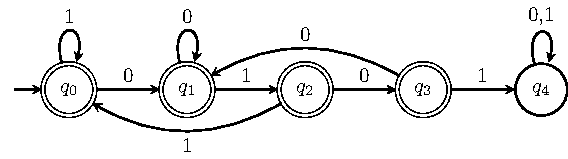
\includegraphics[width=90mm]{29_1}}
    \end{figure}
  \item $L_2=\{0^i1^j0^k\text{ : $i\geq 1, \ k\geq 0, \ i$ impar, $k$ múltiplo de 3 y $j\geq 2$}\}$

    \begin{figure}[H]
      \centering
      \subfigure{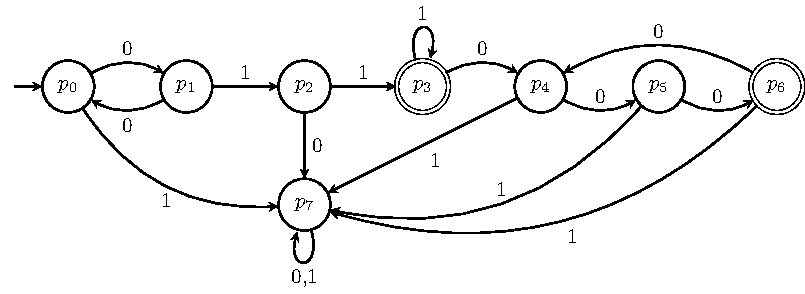
\includegraphics[width=130mm]{29_2}}
    \end{figure}
  \end{itemize}

  Diseñar el AFD minimal que reconoce ($L_2\cap L_1$). \\

  El autómata sin minimizar (sólo agrupando los estados de error) es
  el siguiente.
  
  \begin{figure}[H]
    \centering
    \subfigure{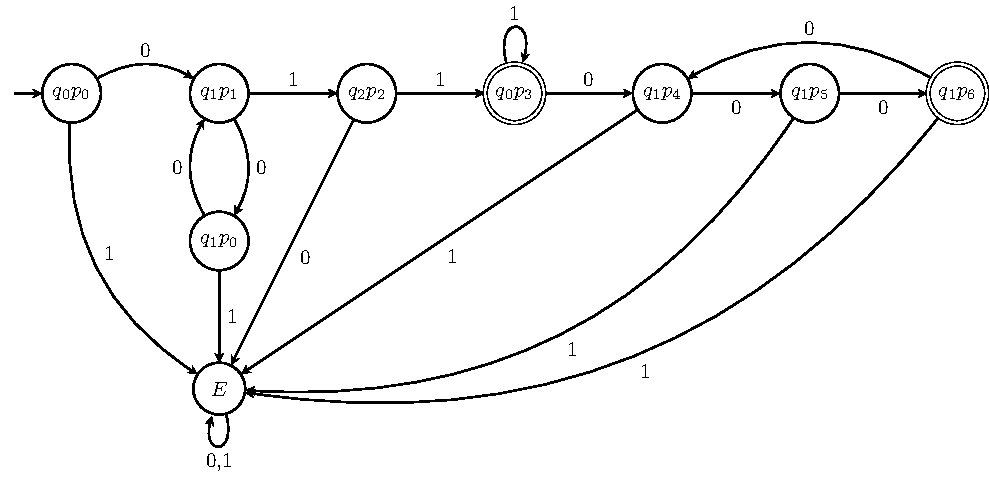
\includegraphics[width=120mm]{29_3}}
  \end{figure}
  
  Tiene sólo dos estados indistinguibles: $q_0p_0$ y $q_1p_0$, luego el
  autómata minimal es el que resulta de agrupar ambos estados.

  \begin{figure}[H]
    \centering
    \subfigure{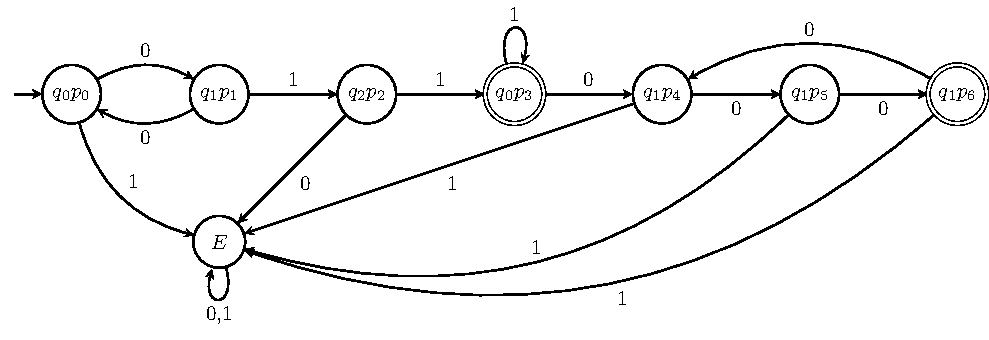
\includegraphics[width=130mm]{29_3_min}}
  \end{figure}

  Podemos apreciar que este autómata es isomorfo al que hemos diseñado
  para $L_2$, lo cual ocurre porque $L_2 \subset L_1$ (es claro que
  las palabras de $L_2$ no tienen a `0101' como subcadena).
\end{exercise}

~

\setcounter{exercise}{44}

\begin{exercise}~ $A=\{0,1,+,=\}$, probar que el lenguaje
  \[ADD=\{x=y+z \ | \ x,y,z \text{ son números en binario y la suma es correcta}\}\]
  no es regular. \\

  Probaré que $ADD$ no satisface el lema de bombeo. Sea
  $n \in \mathbb{N}$, la palabra $1^n=0+1^n$ está en el lenguaje y
  tiene longitud $2n+3 \geq n$. Tomamos una descomposición cualquiera
  de la forma $uvw$ con $|uv| = l \leq n$ y $|v|\geq 1$, por lo tanto
  $v = 1^k$ para algún $k \geq 1$. \\

  La palabra $uv^2w$ será $1^{l-k}1^{2k}1^{n-l}=0+1^n$, que
  simplificando queda $1^{n+k}=0+1^n$. Como $k \geq 1$, el valor
  númerico de $1^{n+k}$ será estrictamente mayor que el de $1^n$, por
  lo tanto la palabra $uv^2w$ no está en $ADD$ (la suma no es
  correcta). \\

  Resumiendo, dado un valor de $n$ cualquiera, podemos encontrar en el
  lenguaje una palabra $z$ de longitud mayor que $n$ tal que para toda
  descomposición de $z$ de la forma $uvw$, la palabra $uv^2w$ no está
  en el lenguaje. Luego  $ADD$ no es regular.
\end{exercise}

\begin{exercise}~ La mezcla perfecta de dos lenguajes $L_1$ y $L_2$
  sobre un alfabeto $A$ se define como
  \[\{w \ | \ w=a_1b_1a_2b_2\ldots a_kb_k \text{ donde } a_1\ldots a_k
    \in L_1, \ b_1\ldots b_k \in L_2, \ a_i,b_i \in A\}\] Demostrar
  que si $L_1$ y $L_2$ son regulares, su mezcla perfecta lo es. \\
  
\end{exercise}

~

\begin{exercise}~ Minimizar el autómata. \\
\vspace{-7mm}
  \begin{figure}[H]
    \centering
    \subfigure{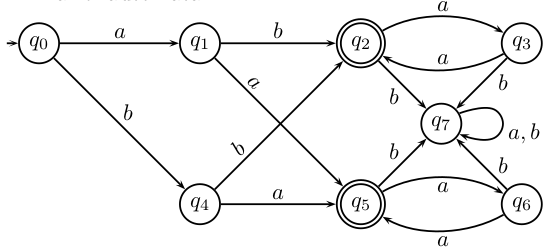
\includegraphics[width=120mm]{47_enunciado}}
  \end{figure}
  \vspace{-7mm}
  
  No hay estados inaccesibles.
  
  Usando el algoritmo visto en clase, he obtenido que las parejas de
  estados indistinguibles son $(q_1,q_4)$, $(q_2,q_5)$ y $(q_3,q_6)$.

  El autómata minimal será el resultante de agrupar cada una de las
  parejas.

  \begin{figure}[H]
    \centering
    \subfigure{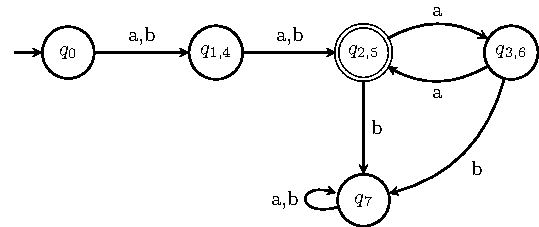
\includegraphics[width=120mm]{47}}
  \end{figure}
  
\end{exercise}

\end{document}
